\section{Experiments}
\label{sec:experiments}

% Table order is deliberate: the MEASURED result (tab:selection) is Table 1, the
% not-yet-run scale sweep (tab:main) is Table 2. At every commit the paper's lead table
% is real data. If this run dies, whatever is pushed is what gets submitted (writing.md
% §4b) — the lead table must never be the fabricated one.
\begin{table}[t]
\centering
\small
\setlength{\tabcolsep}{4pt}
\caption{\textbf{\mname improves recovery under every selection rule.} Fraction of the
plain-skip NLL damage recovered on Qwen2.5-0.5B at matched skipped-layer sets, for three
rules for choosing which $k$ blocks to skip. Positive is better; \emph{negative means the
method is worse than simply dropping the update}. \mname recovers the most damage under
every rule and both budgets, so it can be applied on top of whichever layer-selection
method a practitioner already uses; layer selection is not our contribution, and we do not
propose one. The scalar predictor, by contrast, is catastrophic under the cheapest rule.
Copy Update is worse than plain skipping everywhere. Best value per column in \textbf{bold}. Hardware and protocol: \Cref{sec:app-protocol}.}
\label{tab:selection}
\begin{tabular}{llcc}
\toprule
Selection rule & Predictor & $k=2$ & $k=4$ \\
\multirow{3}{*}{\makecell[l]{Predictability $P_\ell$ \\ \footnotesize(no skipping needed)}}
  & Copy Update            & $-0.779$ & $-1.800$ \\
  & Scalar AR(1)           & $-0.745$ & $-0.128$ \\
  & \textbf{\mname (Ours)} & \textbf{$+0.053$} & \textbf{$+0.194$} \\
\graymidrule
\multirow{3}{*}{\makecell[l]{Lowest single-layer \\ \footnotesize damage (dev set)}}
  & Copy Update            & $-1.736$ & $-2.395$ \\
  & Scalar AR(1)           & $+0.039$ & $+0.040$ \\
  & \textbf{\mname (Ours)} & \textbf{$+0.078$} & \textbf{$+0.074$} \\
\graymidrule
\multirow{3}{*}{\makecell[l]{Measured recovery \\ \footnotesize(dev set)}}
  & Copy Update            & $-0.140$ & $-0.686$ \\
  & Scalar AR(1)           & $+0.166$ & $+0.163$ \\
  & \textbf{\mname (Ours)} & \textbf{$+0.205$} & \textbf{$+0.247$} \\
\bottomrule
\end{tabular}
\end{table}

\begin{table}[t]
\centering
\footnotesize
\setlength{\tabcolsep}{3pt}
\caption{\textbf{Qwen2.5-7B, the deployable operating point.} Downstream quality at
matched skipped-layer sets, layers chosen by measured residual damage, the deployable
rule. Within each budget every predictor skips the \emph{identical} blocks (verified per
run), so differences isolate the update predictor. NLL is lower-better, accuracies
higher-better; the best value in each column within a budget is in \textbf{bold},
whichever method attains it. \mname wins the NLL column at every budget and scale. On accuracy,
\emph{at these light budgets} ($k \le 4$), no difference is statistically significant at any
scale (largest $|z| = 1.18$, against a $95\%$ bar of $1.96$ and a Bonferroni bar of
$3.35$). At heavier budgets the picture changes and the gains become significant
(\Cref{sec:app-pareto}). The point estimates favour Plain Skip on 0.5B and \mname on 7B, and
neither direction clears sampling noise. Gap recovered is the fraction of the
Dense$\rightarrow$Plain Skip \emph{average-accuracy} drop a method restores, reported
with its absolute count in parentheses, net correct answers against Plain Skip, out of
300 graded on 0.5B and 900 on 1.5B and 7B. Read the count, not the fraction:
7B $k{=}4$'s $+35.5\%$ is 22 answers, and is not significant
(\Cref{sec:app-noise}). An empty cell means not applicable: Dense is the reference, and
Plain Skip is $0$ by construction. Hardware and protocol: \Cref{sec:app-protocol}.}
\label{tab:main}
\begin{tabular}{llcccccc}
\toprule
Method & $k/L$ & WikiText-2 NLL $\downarrow$ & HellaSwag $\uparrow$ & PIQA $\uparrow$ & ARC-E $\uparrow$ & Avg. $\uparrow$ & Gap rec. $\uparrow$ \\
\midrule
\multicolumn{8}{c}{\textit{\cellcolor[HTML]{EFEFEF}Qwen2.5-7B ($L=28$)}} \\
\midrule
Dense                  & 0/28 & 1.98 & 80.0 & 79.7 & 78.7 & 79.4 & \\
\graymidrule
Plain Skip             & 2/28 & 2.12 & 73.7 & \textbf{78.3} & 71.0 & 74.3 &  \\
Copy Update            & 2/28 & 2.29 & 68.3 & 73.7 & 59.0 & 67.0 & -143.5\%\ (-66) \\
Scalar AR(1)           & 2/28 & 2.12 & \textbf{74.0} & \textbf{78.3} & 71.3 & 74.6 & +4.3\%\ (+2) \\
\textbf{\mname (Ours)} & 2/28 & \textbf{2.11} & 73.0 & 78.0 & \textbf{73.3} & \textbf{74.8} & +8.7\%\ (+4) \\
\graymidrule
Plain Skip             & 4/28 & 2.38 & 69.0 & 75.7 & 73.0 & 72.6 &  \\
Copy Update            & 4/28 & 2.95 & 58.7 & 68.7 & 53.0 & 60.1 & -180.6\%\ (-112) \\
Scalar AR(1)           & 4/28 & 2.36 & 67.7 & \textbf{78.0} & 73.7 & 73.1 & +8.1\%\ (+5) \\
\textbf{\mname (Ours)} & 4/28 & \textbf{2.29} & \textbf{70.3} & 77.3 & \textbf{77.3} & \textbf{75.0} & +35.5\%\ (+22) \\
\bottomrule
\end{tabular}
\end{table}

\begin{figure*}[t]
\centering
\begin{subfigure}{0.37\textwidth}
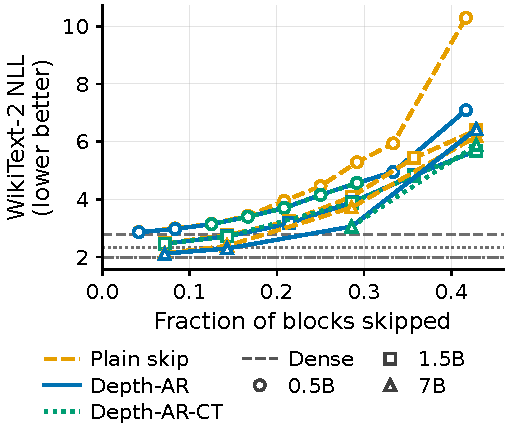
\includegraphics[width=\linewidth]{figures/fig2a_frontier.pdf}
\caption{The quality--compression frontier.}
\label{fig:frontier}
\end{subfigure}
\hfill
\begin{subfigure}{0.37\textwidth}
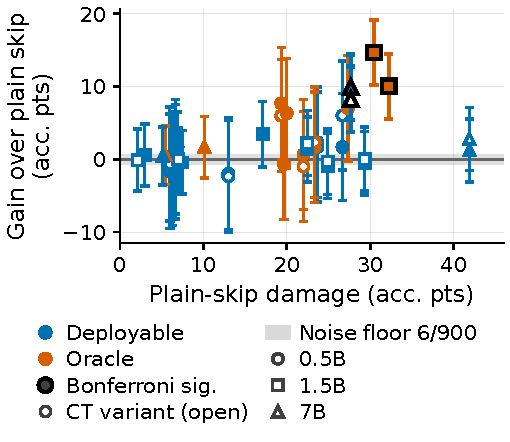
\includegraphics[width=\linewidth]{figures/fig2b_significant_gains.pdf}
\caption{Gain against damage.}
\label{fig:gains}
\end{subfigure}
\caption{\textbf{Significant gains appear only where skipping does severe damage.}
\emph{Left:} WikiText-2 NLL against the fraction of blocks skipped, for Qwen2.5-0.5B (circles),
1.5B (squares) and 7B (triangles), layers chosen by measured residual damage, every predictor
skipping identical blocks. \mname sits below plain skipping at every measured fraction on 0.5B
and 1.5B; dashed lines are the dense models. \emph{Right:} every accuracy comparison in the
paper, plotted as gain over plain skipping against the damage plain skipping does. Bars are
$95\%$ confidence intervals; the grey band is the evaluation's own measured reproducibility
floor, replicated after the main analysis closed (6 answers of 900, or $0.67$ accuracy points,
in BF16; \Cref{sec:app-noise}). Gains sit on zero where damage is small. Every comparison
surviving Bonferroni correction across all 63 tests (filled) lies at the right, at damage above
$27.7$ points, under both the deployable and the recovery-maximising rule. Severe damage is
necessary for a significant gain, and not sufficient: several badly damaged cells show none.
Hardware and protocol: \Cref{sec:app-protocol}.}
\label{fig:gains-pair}
\end{figure*}


\paragraph{Setup.} We evaluate Qwen2.5-0.5B, Qwen2.5-1.5B and Qwen2.5-\topscale
\citep{qwen2025}. Coefficients are fitted in closed form (\cref{eq:fit}) on unlabeled
WikiText-103 \citep{merity2017pointer} and scored on a disjoint held-out split; no task
data is used for calibration. We report NLL and accuracy on HellaSwag
\citep{zellers2019hellaswag}, PIQA \citep{bisk2020piqa} and ARC-Easy
\citep{clark2018think} (100 examples per task on 0.5B, 300 on 1.5B and
\topscale), and give accuracy deltas as absolute counts, since recovered-gap fractions
divide by very small denominators. Skipped blocks are non-adjacent, and within a budget
every predictor skips the \emph{identical} blocks, isolating the predictor from the
selection rule. Full protocol, hardware and precisions in \Cref{sec:app-protocol}. Every accuracy effect is measured against three
quantified uncertainty sources: binomial standard error, Bonferroni correction across the full
family of 63 comparisons, and the evaluation's own measured batch-shape jitter
(\Cref{sec:app-noise}).

\paragraph{A single coefficient per layer is not enough.} \Cref{tab:selection} (\Cref{sec:app-selection}) reports the
fraction of plain-skip NLL damage each predictor recovers under three rules for choosing
which blocks to skip. The scalar predictor of \cref{eq:ar1} is not a mildly weaker \mname:
under the cheap rule it is \emph{worse} than plain skipping, recovering $-0.745$ of
the damage at $k=2$. One coefficient per channel, nothing else changed, turns that into
$+0.053$. \mname recovers more damage than every alternative under \emph{every} rule
and both budgets, so it composes with whichever selection method a practitioner already
uses. Copy Update is worse than plain skipping everywhere, so the benefit comes from
\emph{fitting} the coefficients, not from injecting a nonzero update.

\paragraph{At a matched budget, likelihood recovery grows with scale.} \Cref{tab:main} carries the 7B comparison. At the light, damage-based
operating point \mname recovers
4.6\%, 10.3\% and 23.3\% of the plain-skip damage on 0.5B, 1.5B and 7B at $k=4$. The trend is
budget-specific: at $k=2$ recovery is flat to mildly declining with scale (8.4\%, 8.2\%,
7.3\%), so we claim no general scaling law. The scalar predictor recovers consistently less, and Copy Update is
worse than not predicting at all.

\paragraph{Significant downstream gains appear only where the damage is severe.} Accuracy is
where the skip operator either matters or does not, and what decides which is not the
selection rule but how much damage skipping does. At light budgets, where plain skipping
barely hurts, no accuracy difference is significant at any scale (largest $z=1.18$),
and the differences are smaller than the evaluation's own reproducibility floor. Where the
damage is severe, the gains are large. Under the \emph{deployable} damage-based rule at
28.6\% of blocks skipped on Qwen2.5-7B, \mname answers 89 more questions
correctly out of 900 than plain skipping ($z=4.31$), recovering 38.1\% of
the language-modelling damage and 35.7\% of the accuracy gap. Under damage-seeking
selection on Qwen2.5-1.5B it answers 132 and 90 more ($z=6.45$,
$4.37$). These are 4 of 63 comparisons and the only ones to survive
Bonferroni correction, and every one occurs where plain skipping costs at least 27.7 accuracy
points. Severe damage is \emph{necessary} for a downstream gain and not sufficient: of the six
cells whose damage exceeds 27 points only three gain significantly (\Cref{fig:gains-pair}).
Damage says where repair can pay off, not how much it will.

These are gains over a badly damaged baseline (61.7\% average accuracy against a dense 79.4\%),
not a claim that the compressed model matches dense quality, and the pattern has a limit
(\Cref{sec:app-pareto}).

\paragraph{The forecast is cheap.} On Qwen2.5-7B at four skipped blocks, \mname adds
0.64\% \emph{prefill} latency over plain skipping at sequence length 512, retaining a
1.141$\times$ prefill speedup over the dense model where plain skipping reaches
1.148$\times$ (\Cref{sec:app-latency}). Both methods sit at effectively the same point on
the compute axis, so all of \mname's advantage is quality at that point. Repair the update
when skipping is expensive; do not bother when it is cheap.

Extended results across all scales, budgets, and both model families appear in
\Cref{sec:app-experiments}.

\paragraph{Boundaries.} Two, both reported in full in \Cref{sec:app-noise} and
\Cref{sec:app-qwen3}: at light budgets the accuracy effects are smaller than the evaluation's own
measured reproducibility floor, and in the one out-of-family cell where repair fails
(Qwen3-1.7B), four layers that each repair to better than dense individually fail to compose.

